\section{CÁC HỆ THỐNG LIÊN QUAN}
\subsection{Ristorante Cracco}

\begin{figure}[H]
    \centering
    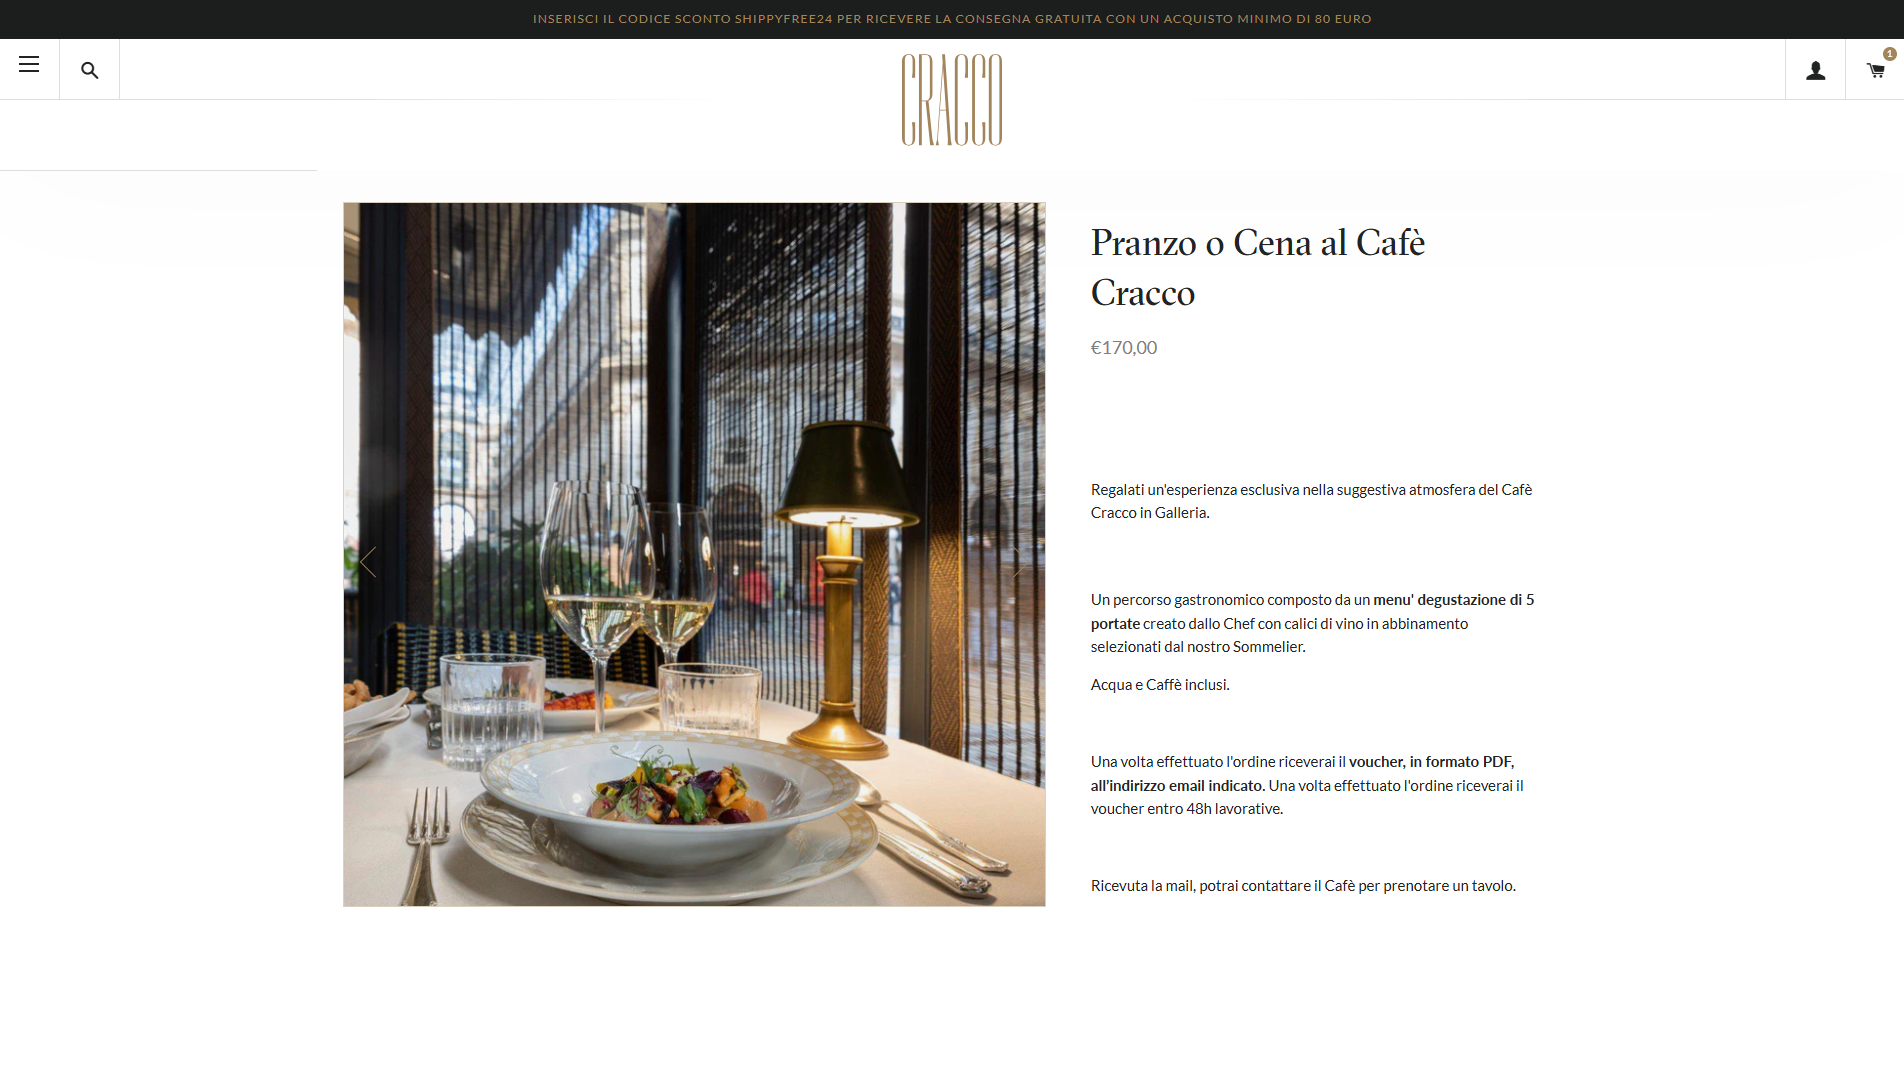
\includegraphics[width=15cm]{Images/ristorante_cracco.png}
    \vspace{0.5cm}
    \caption{Giao diện website Ristorante Cracco. Nguồn: \href{https://www.ristorantecracco.it}{ristorantecracco.it}}
    \label{fig:my_label}
\end{figure}

Ristorante Cracco là một nhà hàng cao cấp tọa lạc tại trung tâm Milano, Ý, trong khu mua sắm lịch sử Galleria Vittorio Emanuele II. Được điều hành bởi đầu bếp danh tiếng Carlo Cracco, nhà hàng mang đến trải nghiệm ẩm thực tinh tế, kết hợp giữa truyền thống và sự sáng tạo hiện đại. Không gian của Ristorante Cracco trải rộng trên nhiều tầng, bao gồm nhà hàng chính, quán cà phê, hầm rượu và khu vực tổ chức sự kiện riêng. Thực đơn đa dạng với các món ăn độc đáo như súp cá bọc vỏ bánh và lòng đỏ trứng ngâm với măng tây và nấm cục đen, cùng với các món truyền thống như risotto nghệ với tủy xương nướng và ragù gan. Hầm rượu của nhà hàng chứa hơn 2.000 nhãn hiệu và hơn 10.000 chai rượu, chủ yếu từ Ý và Pháp. Trang web chính thức của Ristorante Cracco \href{https://www.ristorantecracco.it}{"https://www.ristorantecracco.it"} cung cấp thông tin chi tiết về thực đơn, đặt bàn trực tuyến và các sự kiện đặc biệt, giúp khách hàng dễ dàng tiếp cận và trải nghiệm dịch vụ đẳng cấp của nhà hàng.

\subsection{KFC Việt Nam}

\begin{figure}[H]
    \centering
    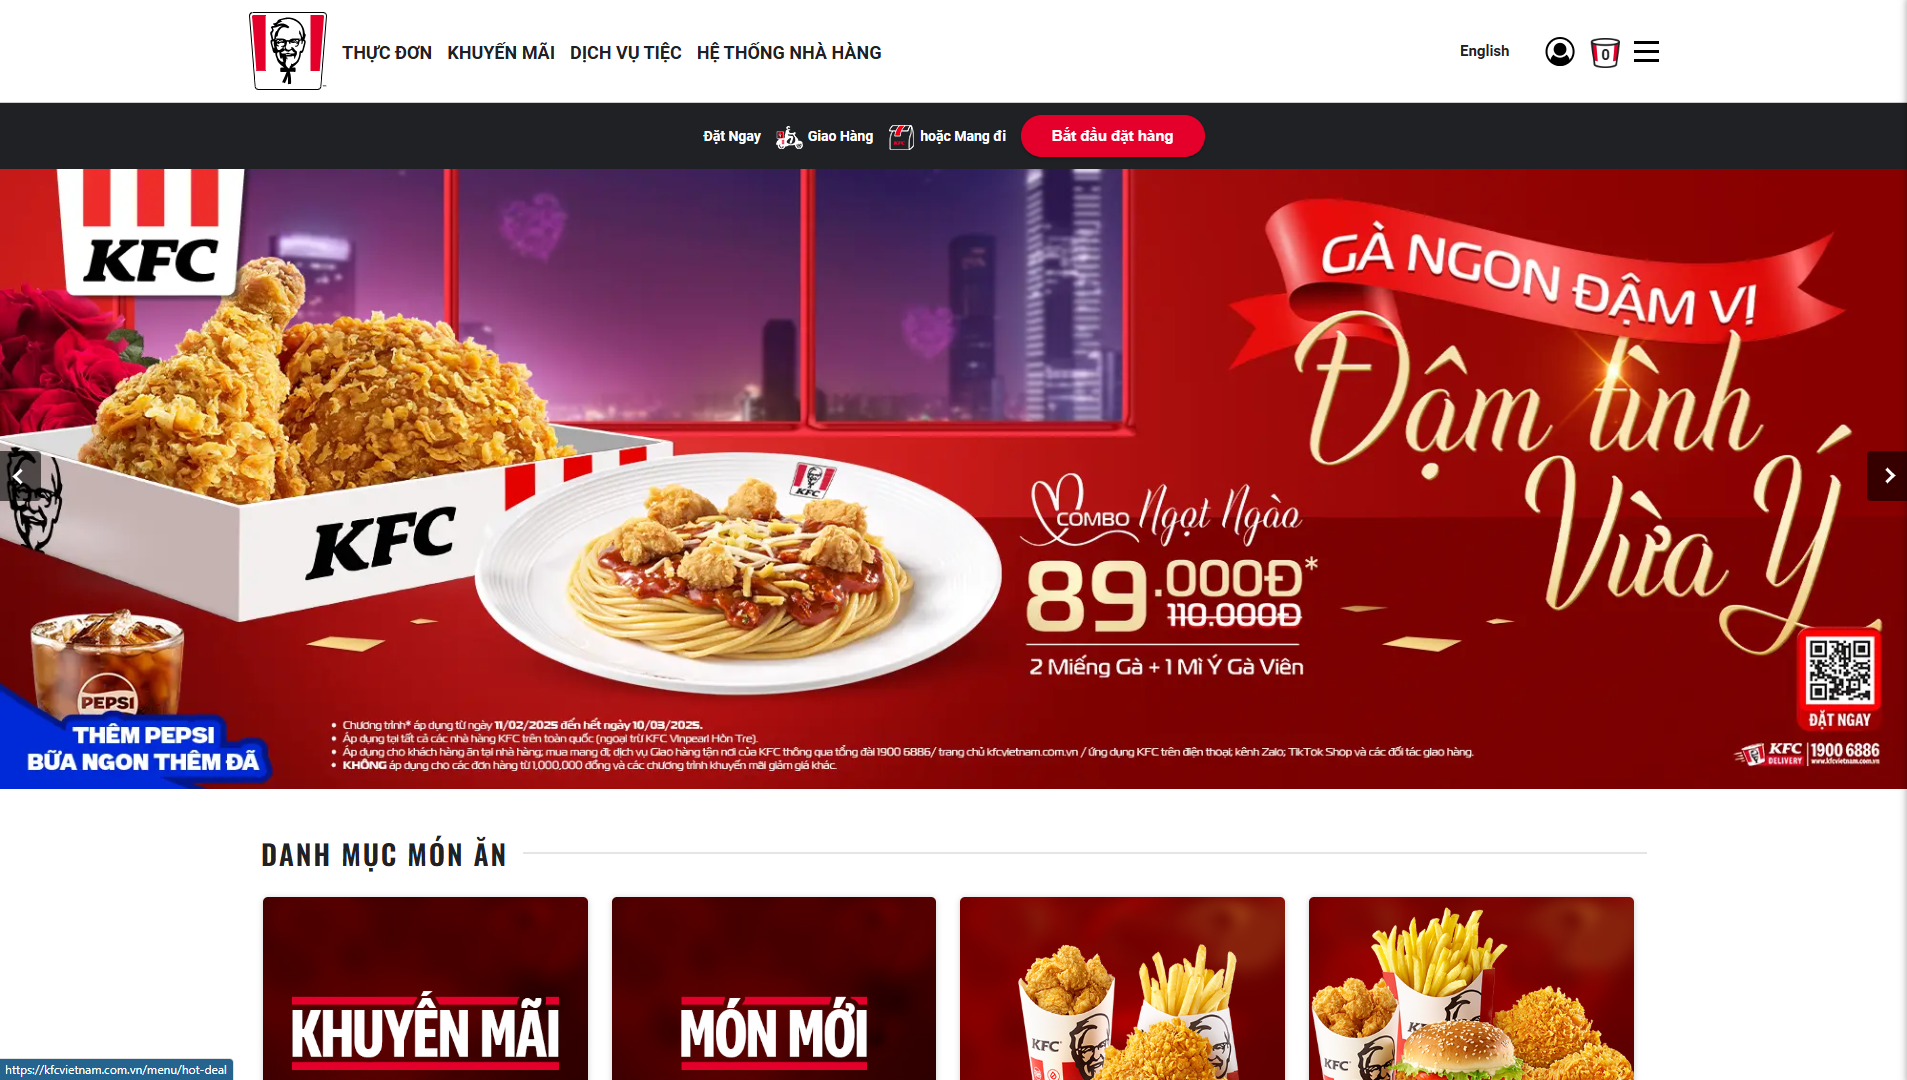
\includegraphics[width=15cm]{Images/kfc.png}
    \vspace{0.5cm}
    \caption{Giao diện website KFC Việt Nam. Nguồn: \href{https://kfcvietnam.com.vn}{kfcvietnam.com.vn}}
    \label{fig:my_label}
\end{figure}

KFC Việt Nam là thành viên của tập đoàn Yum! Brands Inc. (Hoa Kỳ), chuyên cung cấp các sản phẩm gà rán và nướng, cùng với các món ăn kèm và sandwich chế biến từ thịt gà tươi. Kể từ khi khai trương nhà hàng đầu tiên tại TP. Hồ Chí Minh vào năm 1997, KFC đã mở rộng mạng lưới lên hơn 140 nhà hàng trên 21 tỉnh/thành phố, tạo việc làm cho hơn 3.000 lao động. Trang web chính thức của KFC Việt Nam \href{https://kfcvietnam.com.vn}{"https://kfcvietnam.com.vn"} cung cấp thông tin chi tiết về thực đơn đa dạng, bao gồm các món gà rán truyền thống và những món ăn được điều chỉnh phù hợp với khẩu vị Việt như Gà Big'n Juicy, Gà Giòn Không Xương, Cơm Gà KFC và Bắp Cải Trộn. Ngoài ra, trang web còn cập nhật các chương trình khuyến mãi, thông tin về nhà hàng và dịch vụ giao hàng trực tuyến, giúp khách hàng dễ dàng đặt món và tận hưởng hương vị KFC mọi lúc, mọi nơi.

\subsection{Haidilao}

\begin{figure}[H]
    \centering
    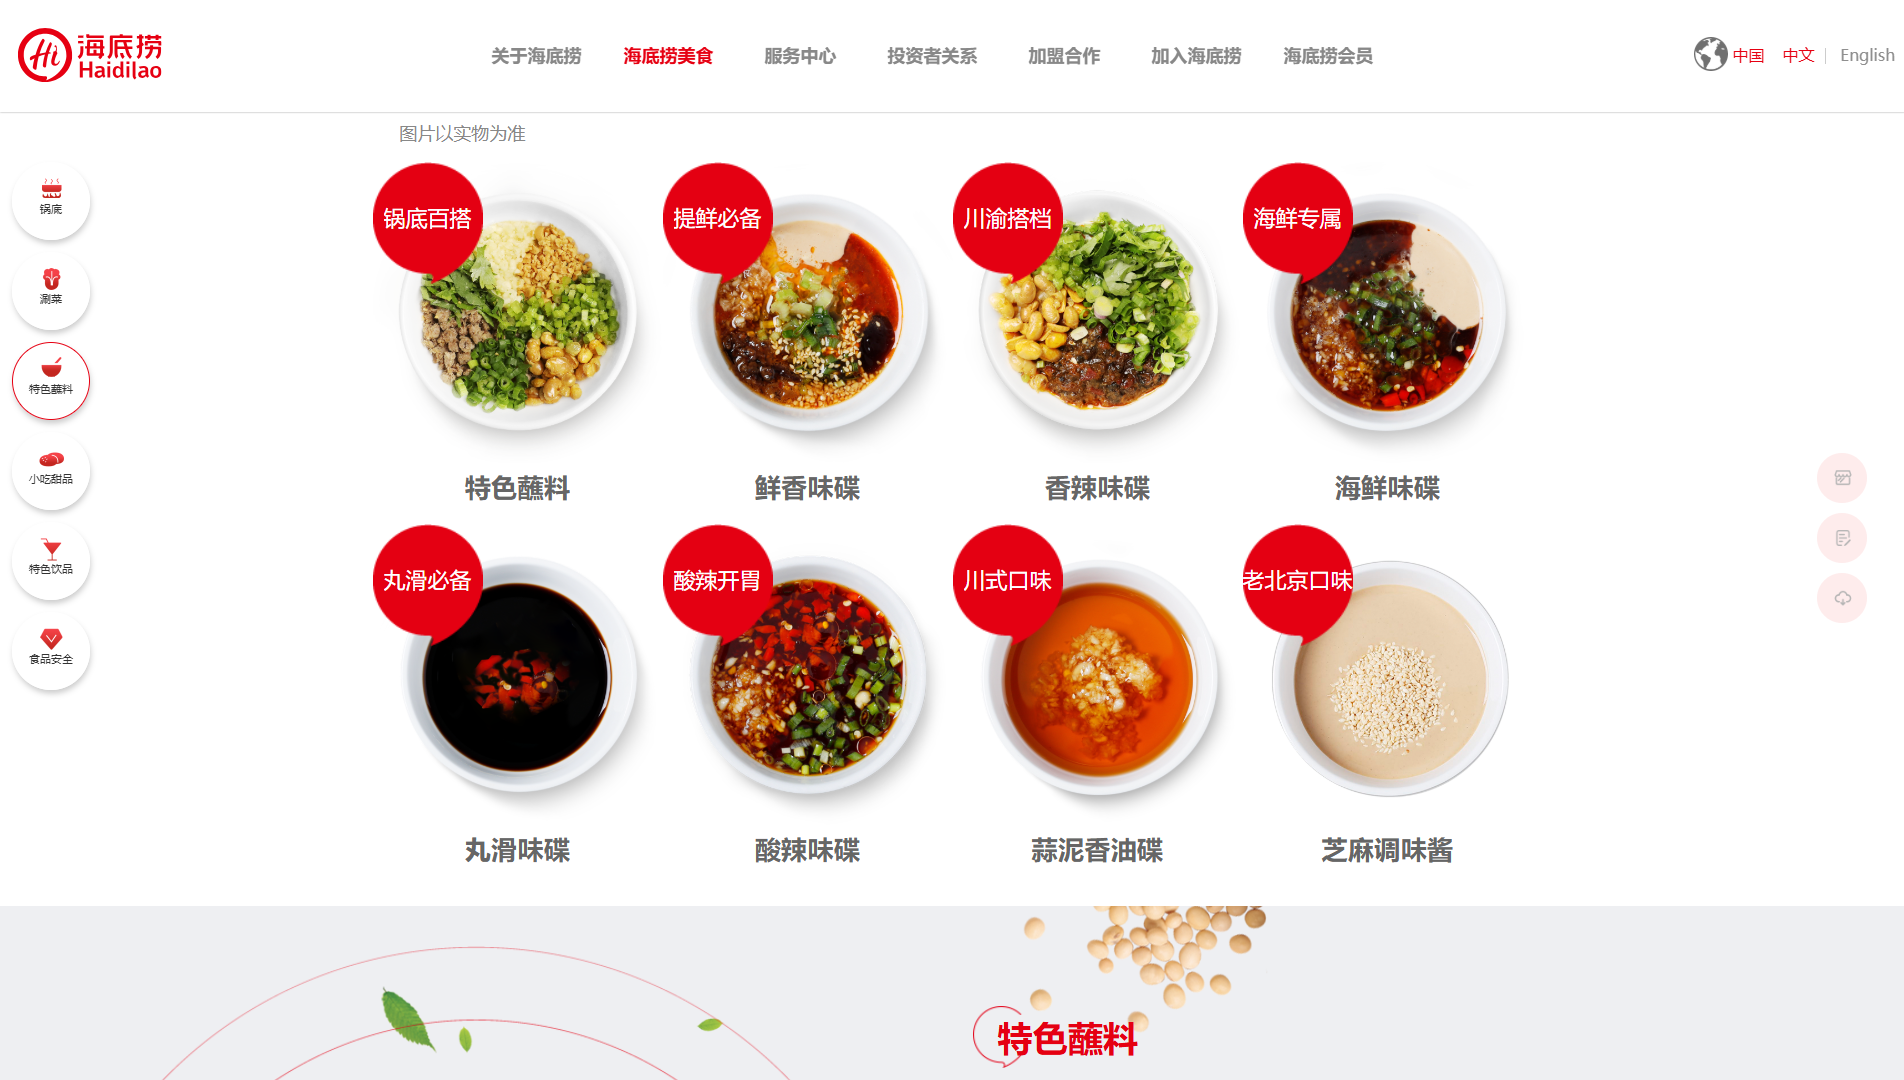
\includegraphics[width=15cm]{Images/haidilao.png}
    \vspace{0.5cm}
    \caption{Giao diện website Haidilao. Nguồn: \href{https://www.haidilao.com}{haidilao.com}}
    \label{fig:my_label}
\end{figure}

Haidilao là chuỗi nhà hàng lẩu nổi tiếng, thành lập năm 1994 tại Giản Dương, Tứ Xuyên, Trung Quốc. Với dịch vụ khách hàng xuất sắc và hương vị lẩu đặc trưng, Haidilao đã mở rộng ra toàn cầu với hơn 1.300 nhà hàng tại nhiều quốc gia, bao gồm Việt Nam. Trang web chính thức của Haidilao \href{https://www.haidilao.com/}{"https://www.haidilao.com"} cung cấp thông tin về thực đơn, địa điểm các chi nhánh và dịch vụ khách hàng, giúp thực khách dễ dàng tiếp cận và trải nghiệm ẩm thực độc đáo của Haidilao.

\subsection{Yoshinoya}

\begin{figure}[H]
    \centering
    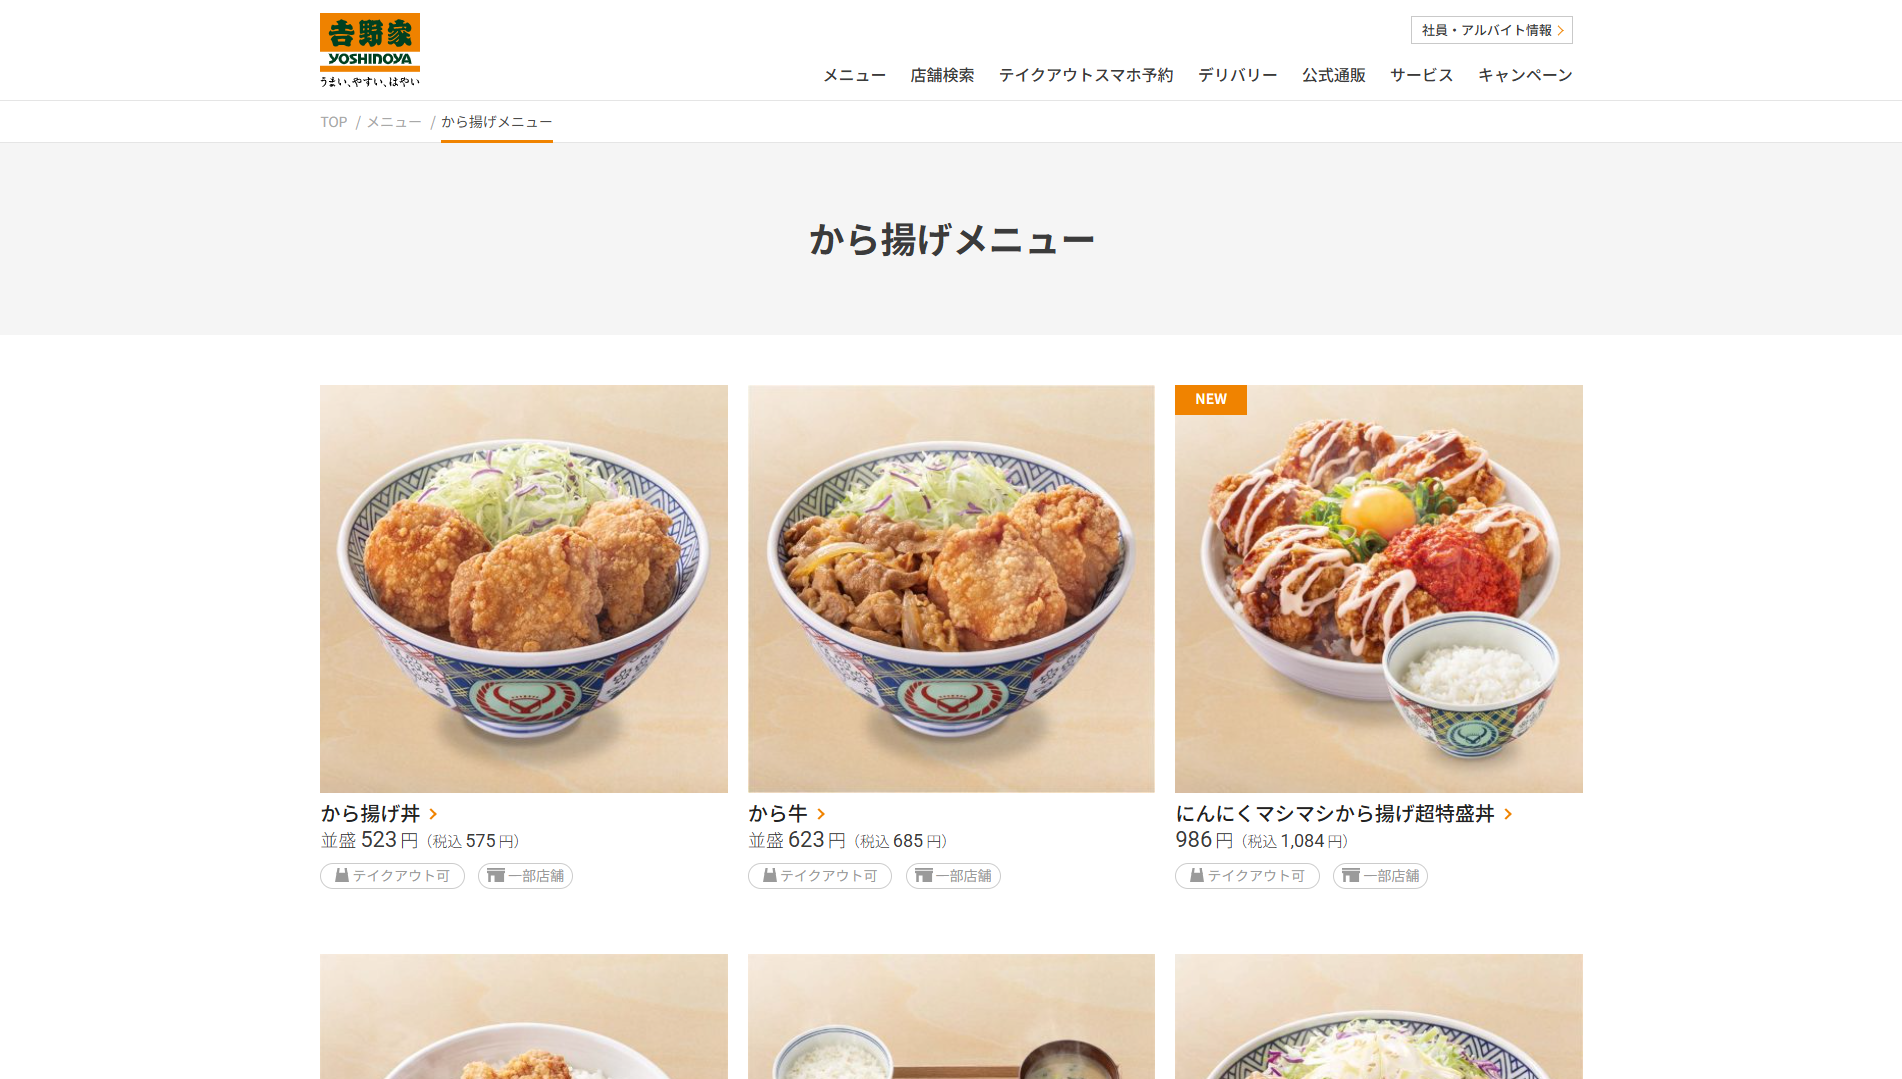
\includegraphics[width=15cm]{Images/yoshinoya.png}
    \vspace{0.5cm}
    \caption{Giao diện website Yoshinoya. Nguồn: \href{https://www.yoshinoya.com}{yoshinoya.com}}
    \label{fig:my_label}
\end{figure}

Yoshinoya là một chuỗi nhà hàng nổi tiếng của Nhật Bản, ra đời từ năm 1899 tại Tokyo, chuyên phục vụ các món ăn truyền thống như gyudon (cơm bò hầm), cơm gà teriyaki và súp miso. Với hơn 120 năm lịch sử, Yoshinoya tự hào mang đến hương vị đậm đà, nguyên liệu tươi ngon và dịch vụ nhanh chóng, tiện lợi. Hiện nay, chuỗi này có mặt tại nhiều quốc gia, trở thành biểu tượng của ẩm thực Nhật Bản đơn giản nhưng tinh tế. Trang web chính thức của Yoshinoya \href{www.yoshinoya.com}{"www.yoshinoya.com"}  giúp khách hàng có thể thưởng thức món ăn yêu thích mọi lúc, mọi nơi thông qua các dịch vụ mà họ cung cấp.

\subsection{Cơm Niêu Sài Gòn}

\begin{figure}[H]
    \centering
    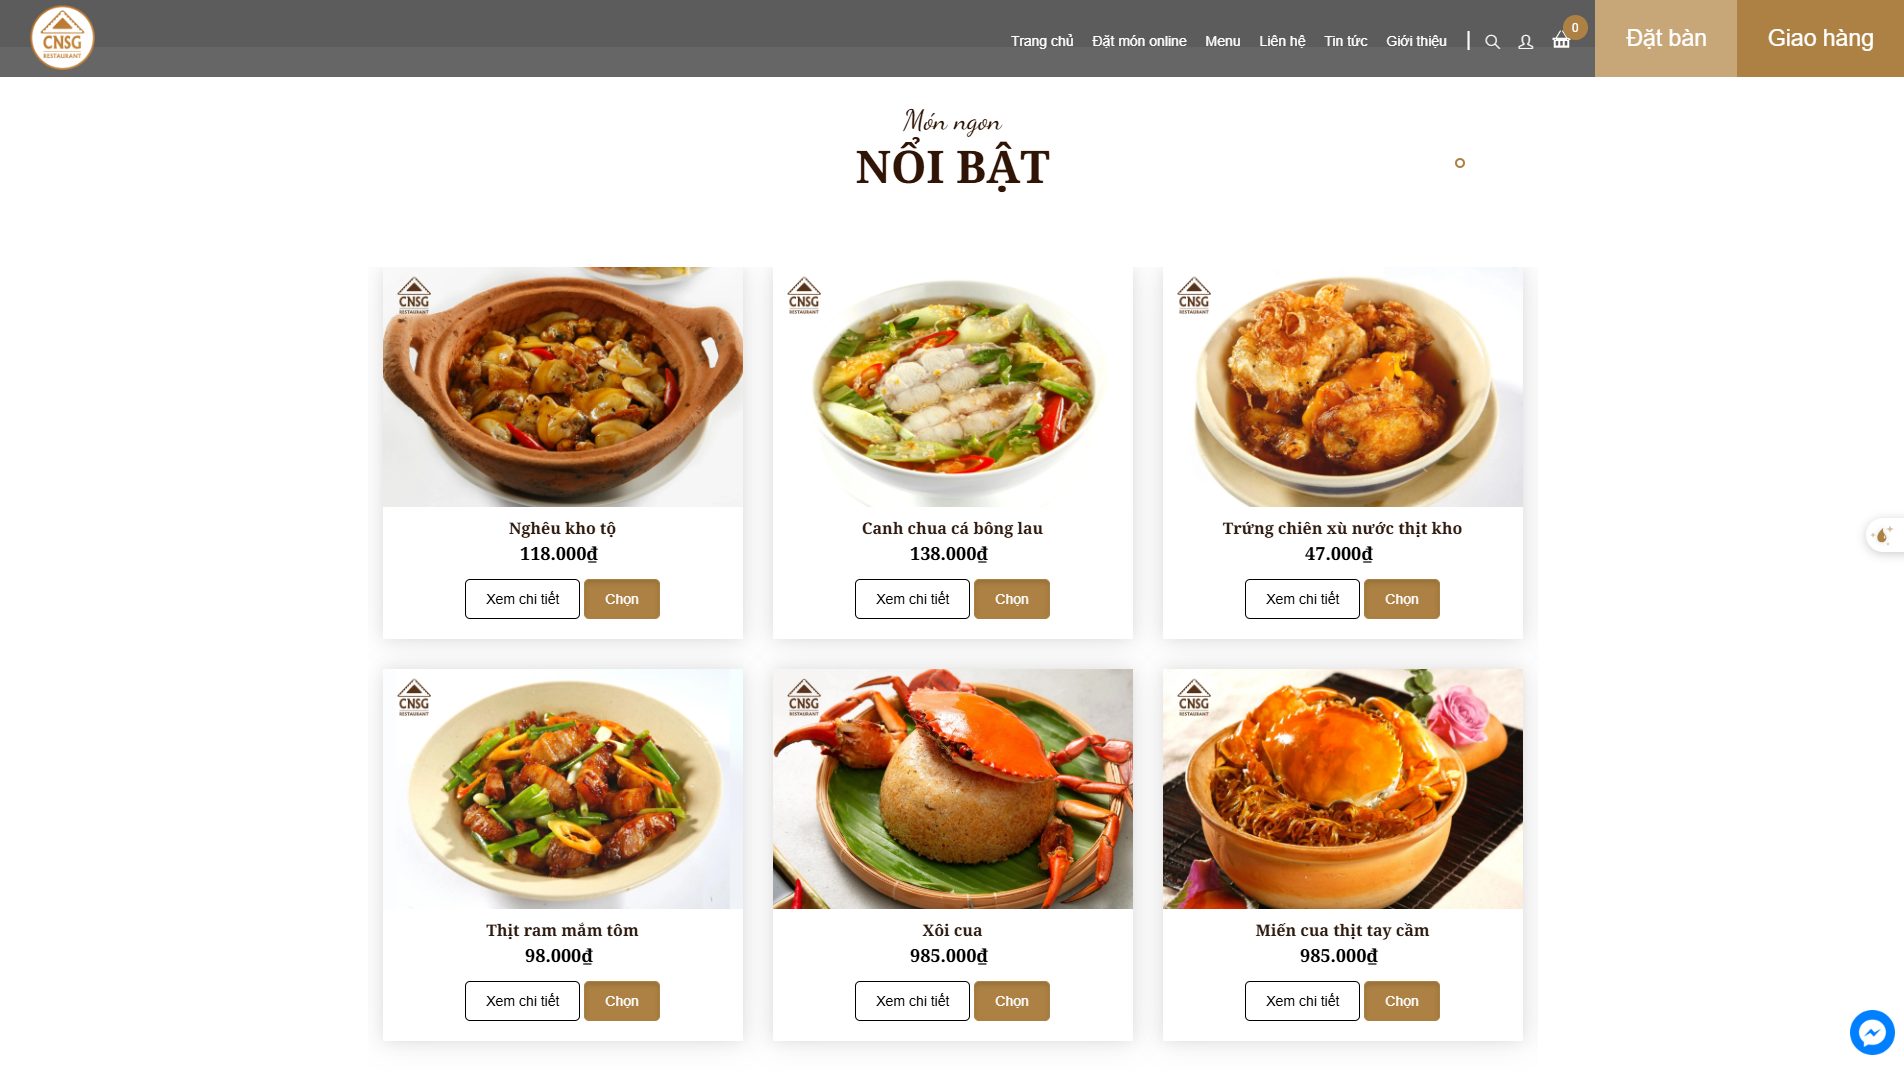
\includegraphics[width=15cm]{Images/comnieusaigon.png}
    \vspace{0.5cm}
    \caption{Giao diện website Cơm niêu Sài Gòn. Nguồn: \href{https://comnieusaigon.com}{comnieusaigon.com}}
    \label{fig:my_label}
\end{figure}

Cơm Niêu Sài Gòn là một địa chỉ ẩm thực truyền thống nổi tiếng qua nhiều thế hệ. Nằm tại quận 3, TP.HCM, nhà hàng thu hút đông đảo khách hàng, đặc biệt là các gia đình và du khách, đến thưởng thức những món ăn đặc sản của miền Nam Việt Nam. Với không gian ấm cúng và thực đơn phong phú, nhà hàng mang đến những bữa ăn đậm đà hương vị quê hương, làm hài lòng cả những thực khách khó tính nhất. Bạn có thể khám phá thêm về thực đơn và dịch vụ của nhà hàng qua trang web chính thức của Cơm Niêu Sài Gòn tại \href{https://comnieusaigon.com}{"https://comnieusaigon.com"}.

\subsection{Thanh's Deli}

\begin{figure}[H]
    \centering
    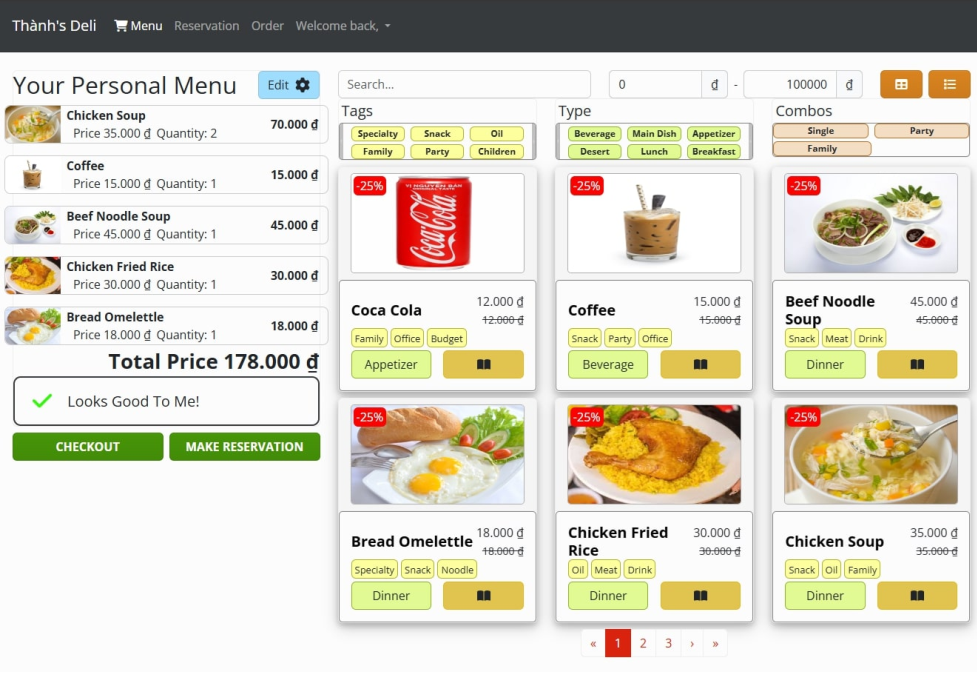
\includegraphics[width=15cm]{Images/thanhsdeli.png}
    \vspace{0.5cm}
    \caption{Giao diện website Thanh's Deli}
    \label{fig:my_label}
\end{figure}

Thanh's Deli là một hệ thống quản lý đặt món và đặt bàn trực tuyến được phát triển bởi Nguyễn Duy Thành trong khuôn khổ đồ án tốt nghiệp. Hệ thống được thiết kế nhằm nâng cao trải nghiệm người dùng tại nhà hàng, giúp khách hàng dễ dàng thực hiện các thao tác đặt món và đặt bàn qua nền tảng trực tuyến.
% % % % % % % 
\subsection{So sánh với hệ thống của nhóm}

Chúng em sẽ tiến hành so sánh hệ thống của mình với các hệ thống khác trong ngành, tập trung vào các chức năng mà họ cung cấp cho khách hàng. Cụ thể, chúng em sẽ đánh giá các nội dung trên trang web của họ, cách thức trình bày các thông tin đó và mức độ tương tác giữa người dùng và hệ thống.

Chúng em sẽ kiểm tra xem các hệ thống có cung cấp 10 nội dung sau đây không: Giới thiệu, Thực đơn, Đặt món trực tuyến, Đặt bàn, Đánh giá và bình luận, Khuyến mãi, Thông tin liên hệ, Đăng nhập/Tài khoản cá nhân, Tương thích di động, và Hỗ trợ khách hàng. Chúng em sẽ đánh giá cách thức trình bày và mức độ hoàn thiện của từng nội dung theo các cấp độ phân loại chi tiết dưới đây:

        \begin{enumerate}
            \item Giới thiệu
                \begin{itemize}
                    \item Cấp độ 1: Cung cấp thông tin cơ bản về nhà hàng (tên, địa chỉ).
                    \item Cấp độ 2: Bao gồm thông tin cơ bản cùng với lịch sử, sứ mệnh và tầm nhìn của nhà hàng.
                    \item Cấp độ 3: Ngoài các thông tin trên, còn có câu chuyện thương hiệu, giới thiệu đội ngũ quản lý và đầu bếp, cùng các giải thưởng đã đạt được.
                \end{itemize}
            \item Thực đơn
                \begin{itemize}
                    \item Cấp độ 1: Danh sách các món ăn và đồ uống cơ bản.
                    \item Cấp độ 2: Thực đơn kèm theo mô tả chi tiết và giá cả cho từng món.
                    \item Cấp độ 3: Thực đơn bao gồm hình ảnh chất lượng cao cho mỗi món, thông tin về nguyên liệu và giá trị dinh dưỡng.
                \end{itemize}
            \item Đặt món trực tuyến
                \begin{itemize}
                    \item Cấp độ 1: Thực đơn sẽ có phần riêng để khách hàng thêm món ăn vào đơn hàng của mình.
                    \item Cấp độ 2: Có hệ thống giỏ hàng cho phép khách hàng có thể coi lại những món ăn trước khi tạo đơn.
                    \item Cấp độ 3: Cho phép thanh toán trực tuyến thông qua các hình thức thanh toán online.
                \end{itemize}
            \item Đặt bàn
                \begin{itemize}
                    \item Cấp độ 1: Cho phép đặt bàn thông qua form cơ bản.
                    \item Cấp độ 2: Hiển thị trạng thái bàn và cập nhật trạng thái theo thời gian thực.
                    \item Cấp độ 3: Cung cấp sơ đồ chi tiết của nhà hàng, cho phép người dùng xem tổng quan các vị trí bàn còn trống.
                \end{itemize}
            \item Đánh giá và bình luận
                \begin{itemize}
                    \item Cấp độ 1: Cho phép nhìn thấy những bình luận do nhà hàng thu thập được, nhưng không cho phép bình luận trực tiếp trên hệ thống.
                    \item Cấp độ 2: Cho phép khách hàng đánh giá, bình luận trực tiếp và nhận phản hồi từ quản lý nhà hàng.
                \end{itemize}
            \item Khuyến mãi
                \begin{itemize}
                    \item Cấp độ 1: Giảm giá cho một món ăn cụ thể với mức giảm cố định.
                    \item Cấp độ 2: Cho phép sử dụng mã giảm giá hoặc voucher.
                    \item Cấp độ 3: Cung cấp chương trình tích điểm dành cho khách hàng thân thiết.
                \end{itemize}
            \item Thông tin liên hệ
                \begin{itemize}
                    \item Cấp độ 1: Chỉ cung cấp địa chỉ và số điện thoại.
                    \item Cấp độ 2: Thêm email liên hệ và bản đồ chỉ đường.
                    \item Cấp độ 3: Có form liên hệ trực tuyến, liên kết với mạng xã hội và hỗ trợ chat trực tiếp.
                \end{itemize}
            \item Đăng nhập/Tài khoản cá nhân
                \begin{itemize}
                    \item Cấp độ 1: Cho phép tạo tài khoản, không dùng mạng xã hôi.
                    \item Cấp độ 2: Cho phép dùng mạng xã hôi để đăng nhập.
                    \item Cấp độ 3: Tài khoản cá nhân cho phép xem lịch sử đặt hàng, nhận ưu đãi dành riêng và quản lý thông tin cá nhân.
                \end{itemize}
            \item Tương thích di động
                \begin{itemize}
                    \item Cấp độ 1: Hiển thị trên di động nhưng chưa tối ưu giao diện và chức năng.
                    \item Cấp độ 2: Tương thích hoàn toàn với thiết bị di động, giao diện và chức năng được tối ưu hóa.
                \end{itemize}
            \item Hỗ trợ khách hàng
                \begin{itemize}
                    \item Cấp độ 1: Cung cấp số điện thoại hỗ trợ chỉ trong giờ hành chính (ví dụ: 8h-17h). Khách hàng có thể gọi khi cần hỗ trợ về các vấn đề cơ bản như đặt món, thắc mắc về dịch vụ.
                    \item Cấp độ 2: Cung cấp email hỗ trợ, khách hàng có thể gửi yêu cầu qua email về các vấn đề cần giải đáp, và nhận phản hồi trong vòng 24 giờ. Hỗ trợ các vấn đề liên quan đến đơn hàng, thanh toán hoặc yêu cầu thông tin thêm về dịch vụ.
                    \item Cấp độ 3: Hỗ trợ khách hàng qua nhiều kênh (chat trực tuyến, email, điện thoại, form liên hệ) với phản hồi nhanh chóng 24/7. Khách hàng có thể liên hệ bất cứ lúc nào để giải quyết các vấn đề khẩn cấp như yêu cầu thay đổi đơn hàng, khiếu nại, hay cần trợ giúp về dịch vụ trong suốt quá trình sử dụng.
                \end{itemize}
        \end{enumerate}

        \begin{longtable}{|p{2cm}|p{1.5cm}|p{1.5cm}|p{1.5cm}|p{1.5cm}|p{1.5cm}|p{1.5cm}|p{1.5cm}|}
        \hline
        \textbf{Chức năng} & \textbf{Menu+ (Our System)} & \textbf{Cracco} & \textbf{KFC} & \textbf{Haidilao} & \textbf{Yoshinoya} & \textbf{Cơm Niêu Sài Gòn} & \textbf{Thanh's Deli}\\ 
        \hline
        \endfirsthead
        \hline
        \textbf{Chức năng} & \textbf{Menu+ (Our System)} & \textbf{Cracco} & \textbf{KFC} & \textbf{Haidilao} & \textbf{Yoshinoya} & \textbf{Cơm Niêu Sài Gòn} & \textbf{Thanh's Deli} \\
        \endhead
        \hline
        % \multicolumn{8}{|r|}{\small\slshape Còn tiếp} \\ \hline
        \endfoot
        \hline
        \endlastfoot
        Giới thiệu & 3 & 2 & 3 & 3 & 3 & 3 & 3\\ 
        \hline
        Thực đơn & 3 & 2 & 3 & 2 & 3 & 2 & 2\\ 
        \hline
        Đặt món trực tuyến & 3 & 0 & 3 & 3 & 3 & 3 & 3\\ 
        \hline
        Đặt bàn & 3 & 1 & 1 & 1 & 2 & 1 & 3\\ 
        \hline
        Đánh giá và bình luận & 2 & 0 & 0 & 0 & 2 & 0 & 2\\ 
        \hline
        Khuyến mãi & 2 & 2 & 3 & 3 & 2 & 2 & 2\\ 
        \hline
        Thông tin liên hệ & 3 & 1 & 3 & 2 & 3 & 3 & 2\\ 
        \hline
        Đăng nhập/Tài khoản cá nhân & 3 & 3 & 3 & 3 & 1 & 3 & 1\\ 
        \hline
        Tương thích di động & 2 & 2 & 2 & 2 & 2 & 2 & 2\\ 
        \hline
        Hỗ trợ khách hàng & 2 & 2 & 3 & 2 & 1 & 2 & 2\\ 
        \hline
        \caption{Bảng so sánh các nhà hàng}\\
        \end{longtable}

\subsection{Kết luận}
Việc so sánh hệ thống của nhóm với các hệ thống hiện có trong ngành nhà hàng đã giúp làm rõ những ưu điểm và nhược điểm của sản phẩm mà nhóm phát triển. Hệ thống của nhóm nổi bật với một số điểm mạnh quan trọng khi so sánh với các hệ thống liên quan.

Đầu tiên, hệ thống của chúng em được cải tiến với khả năng tích hợp các tính năng như tự gọi món qua ứng dụng và thanh toán trực tuyến. Mặc dù các hệ thống như Cơm Niêu Sài Gòn, KFC và Haidilao cũng đã triển khai các tính năng đặt món trực tuyến và thanh toán, nhưng hệ thống của nhóm mang đến một trải nghiệm người dùng dễ dàng và nhanh chóng hơn nhờ vào giao diện thân thiện và tiện lợi. Hơn nữa, hệ thống của nhóm cung cấp phản hồi thời gian thực và khả năng theo dõi đơn hàng một cách thuận tiện, điều mà một số hệ thống khác còn thiếu sót.

Mặc dù hệ thống của chúng em có những ưu điểm về việc tối ưu trải nghiệm người dùng và quy trình, song so với các hệ thống như Yoshinoya hay KFC, hệ thống của nhóm vẫn còn hạn chế về tính linh hoạt trong việc mở rộng các tính năng phức tạp hơn, như tích hợp chương trình khách hàng thân thiết hay quản lý các chương trình khuyến mãi phức tạp. Các tính năng như phân tích hành vi mua sắm và khuyến mãi dựa trên tần suất vẫn là những lĩnh vực cần cải tiến.

Tóm lại, hệ thống của chúng em thể hiện sự vượt trội trong việc tối ưu hóa quy trình đặt món và thanh toán, giúp nâng cao hiệu quả công việc và cải thiện trải nghiệm khách hàng. Tuy nhiên, để có thể phát triển mạnh mẽ hơn, hệ thống cần học hỏi và cải tiến thêm ở những lĩnh vực mở rộng tính năng và quản lý khách hàng. Việc so sánh này đã giúp nhóm nhận diện rõ các điểm mạnh hiện tại cũng như những khu vực cần cải thiện, làm cơ sở để phát triển hệ thống trong tương lai.






